% !TEX root = ../thesis.tex

\chapter{Experiment Results}

In this chapter, the evaluation results are shared, and the three research questions are answered. Similar to the experiment setup, which is divided into three stages, the experiment results are divided into three sections, namely \textit{Clustering Results Evaluation}, \textit{Survey Results Evaluation}, and \textit{Precision Analysis Results}. A few experiment results are separately shared according to different sizes of the candidate document pool. Moreover, the ineffectiveness of certain experiment results is assessed with possible reasons. The section \textit{Precision Analysis Results} shares the outcome of the exploratory analysis and literature comparison.

\section{Clustering Results Evaluation}

As the test set contains 17 user queries and the clustering analysis is performed on each query, and the output is analyzed based on the mean values of the clustering output. Two candidate pools are generated for each query with sizes 30 and 100, respectively. The small candidate pool, \textit{CP-30}, and the large candidate pool, \textit{CP-100}, represent the retrieved results of the original query from both syntactic and semantic matching. \textit{CP-30} contains a maximum of 30 labeled documents. \textit{CP-100} contains around 100 documents, and only a few documents present in the test set are labeled. Therefore, more than half of the \textit{CP-100} documents are unlabeled. The unlabeled documents are removed from the clustering output during the analysis, and only the labeled documents are used for evaluation. This assumes that having more documents in \textit{CP-100} helps to provide better clusters compared to \textit{CP-30}. Furthermore, it is expected to extract better sub-topics from the larger collection in order to gain deeper insights into the data.

\subsection{Clustering Output Analysis}

The sub-topic modeling pipeline is tested on all the hyperparameters of clustering mentioned in Section 6.4.3. Ideally, there should be 1,710 cases to test the clustering output for small and large candidate pools. However, a few test cases have produced very low clustering (only one cluster) and are not considered in the parameter selection. Ultimately, 1,588 and 1,009 possible hyperparameter combinations are evaluated for large and small candidate pools, respectively. The clustering output, consisting of the evaluation metrics, is expressed as the mean over all 17 queries. Furthermore, the analysis is shared separately for the small and large candidate pools. In the analysis below, "silhouette score" denotes the intrinsic evaluation metric, and "targeted negative document ratio" signifies the extrinsic evaluation metric that denotes the quality of separation between relevant and irrelevant clusters.

\ac{HDBSCAN} clustering does not require any parameter to specify the number of clusters created from the data. On the other hand, other parameters need to be well chosen to generate better clusters. Before evaluating the parameters that significantly affect the clustering output, the relation between the evaluation metrics and the number of clusters is analyzed.  \prettyref{fig:silhouette_score_vs_cc} shows the relationship between the silhouette score and the number of clusters. The data is generated when all the hyperparameter possibilities of the clustering pipeline are tested over the test set queries.

\begin{figure}[h]
	\centering
	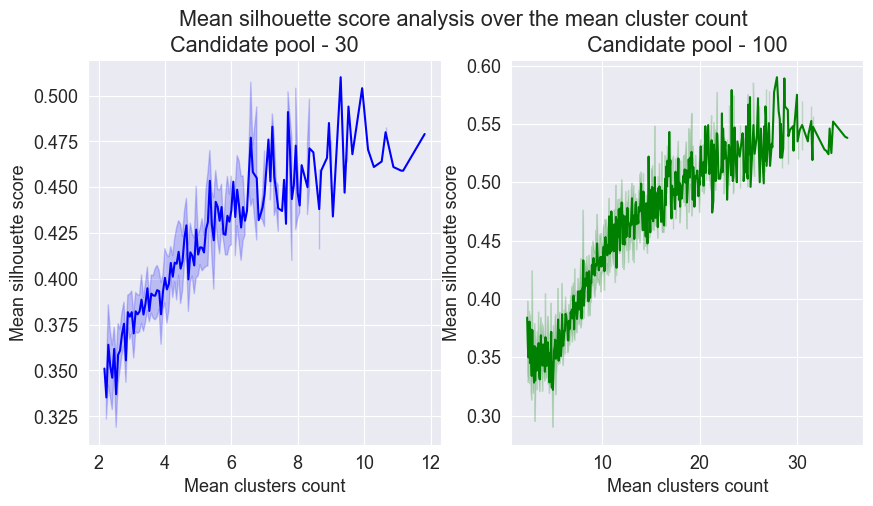
\includegraphics[width=.99\textwidth]{images/subplots/sil_score_ccnt_subplot.png}
	\caption{Silhouette score analysis over clusters count. \label{fig:silhouette_score_vs_cc}}
\end{figure}

The objective of this analysis is to observe whether the number of clusters has an impact on the silhouette score globally. This means that the overall effect of cluster counts is not specific to a particular query or a hyperparameter set. It is clear from \prettyref{fig:silhouette_score_vs_cc} that a relatively high number of clusters generates higher silhouette scores, implying better cluster quality. However, many clusters in both small and large candidate pools (30 and 100) show lower silhouette scores than the highest value. This signifies that a high number of clusters can result in many clusters with very few data points, reducing the quality of clustering as the silhouette score is based on intra- and inter-cluster distances. The best clustering can be achieved when the intra-cluster distance is minimized and the inter-cluster distances are maximized. Therefore, a small number of clusters leads to overlapping clusters (very close) and is not a good choice for clustering parameter selection.

\begin{figure}[h]
	\centering
	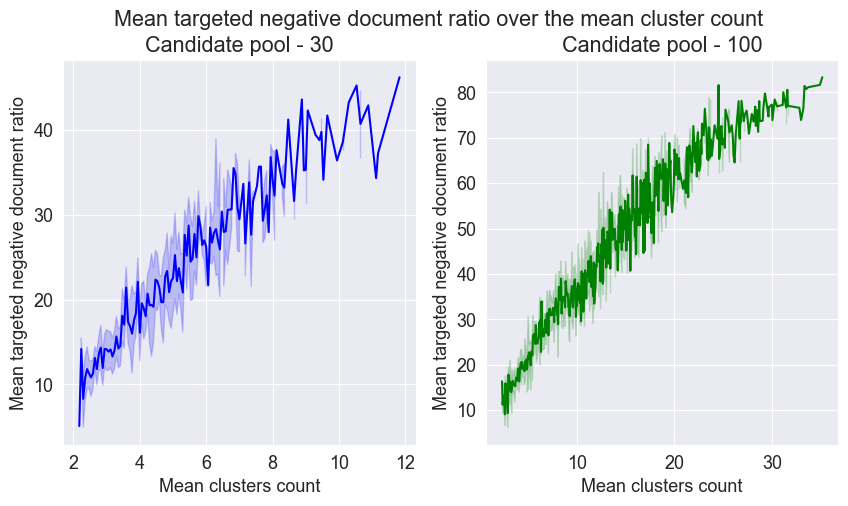
\includegraphics[width=.99\textwidth]{images/subplots/targetfn_score_ccnt_subplot.png}
	\caption[Targeted negative document ratio analysis.]{Targeted negative document ratio analysis over cluster count.  \label{fig:target_function_vs_cc}}
\end{figure}


It is assumed that the heterogeneity or diversity of clusters can be derived from the cluster quality, and to have a wide variety of clusters, the parameters that create a high number of clusters must be selected. One major drawback of this analysis is the combination of all the clustering outputs for all 17 queries in the test set. Some queries generate a low number of clusters, while others generate a high number of clusters. Combining all queries into one analysis may lead to misleading results in certain scenarios. However, since the focus is on observing the overall impact of the number of clusters, the analysis can still be considered for parameter selection without any issues.

\mycomment{
	~\prettyref{tab:correlation_data} shows the Pearson correlation
	over all the hyperparameters tested, and there is a positive correlation between the cluster
	count and evaluation metrics chosen.
	
	\begin{center}
		\captionof{table}{Pearson correlation between the clustering observations.}\label{tab:correlation_data}
		\begin{tabularx}{.99\textwidth}{|Y|c|c|}
			\hline
			Parameter & CP-30 & CP-100 \\
			\hline
			Mean silhouette score and mean clusters count & 0.71 & 0.89 \\
			\hline
			Mean targeted negative document ratio and mean clusters count & 0.76 & 0.94 \\
			\hline
		\end{tabularx}
\end{center}}

 
\prettyref{fig:target_function_vs_cc} shows the relationship between the targeted negative document score and the number of clusters. Similar to the silhouette score, a higher cluster count positively correlates with the targeted document ratio. The design of this evaluation metric slightly favors clustering outputs with a high cluster count, as it creates many clusters with a low number of data points and results in greater separation between clusters. Consequently, fewer clusters indicate poorer cluster quality due to inadequate separation between the documents. Therefore, this metric needs to be relatively higher in order to create a diverse set of clusters with good separation. The large candidate pool has a better silhouette score and targeted negative document ratio compared to the smaller one. Since the labels for all the documents in the large candidate pool are unknown, the actual scores could be even higher than those presented.

\subsection{Candidate Keyword Selection Analysis}
This section explores the impact of the Candidate keyword selection ($cks$) parameter on the clustering output, specifically regarding keyword selection. This analysis is crucial for finalizing the parameter selection. The $cks$ parameter ranges from 10 to 100, with values incrementing by 5, signifying the percentile selection based on query similarity. The similarity score of the $x$ percentile indicates that the score is higher than $x$ percent of the population or the similarity is lower than $100-x$ percent of the population. In the case of $cks$-based selection, only the keywords that are not similar to the query are selected. For example, $cks$ = 60 denotes the selection of keywords with query similarity less than the 60th percentile similarity and the removal of keywords higher than the 60th percentile. Similarly, a value of $cks$ = 100 represents the selection of all keywords without any removal. The keyword selection for a given $cks$ parameter is illustrated in Table \ref{tab:cks_selection}.

\begin{center}
	\captionof{table}{Different $cks$ parameter examples.}\label{tab:cks_selection}
	\begin{tabularx}{.8\textwidth}{|c|Y|}
		\hline
		Cks parameter  &  Selected keywords  \\
		\hline
		
		\textbf{100}  &            All keywords are selected   \\ \hline
		75 &            Keywords with query similarity lower than 75 percentile  \\ \hline
		50 &            Keywords with query similarity lower than 50 percentile  \\ \hline
		25 &            Keywords with query similarity lower than 25 percentile   \\ \hline
		10 &            Keywords with query similarity lower than 10 percentile \\ \hline
		
	\end{tabularx}
	
\end{center}

The keywords selected using the $cks$ parameter are further clustered using \ac{HDBSCAN}. One of the main objectives of this master thesis is to test the effectiveness of clustering with keyword selection compared to no selection. The data used in this analysis is generated from the clustering results for all the possible parameter combinations in the hyperparameter set over the test set queries. The x-axis represents the candidate keyword selection, and the y-axis represents the mean of the respective evaluation metrics.


\begin{figure}[h]
	\centering
	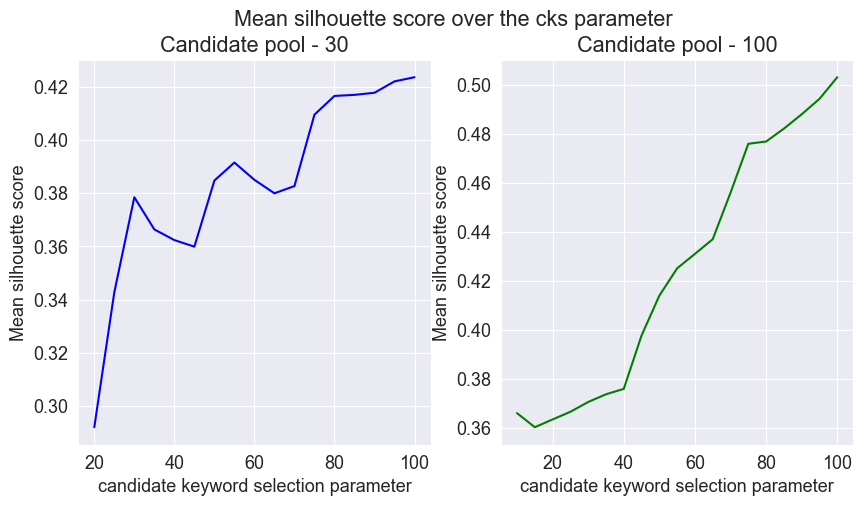
\includegraphics[width=.99\textwidth]{images/subplots/csk_sil_score_subplot.png}
	\caption[Silhouette score analysis over cks parameter.]{Silhouette score analysis over candidate keyword selection parameter. \label{fig:silhouette_score_vs_csk}}
\end{figure}  

 \prettyref{fig:silhouette_score_vs_csk} presents the relationship between the mean silhouette score and the $cks$ parameter. Results from the large candidate pool clearly show that a higher $cks$ parameter generates a better mean silhouette score. This signifies that selecting a lower number of keywords is better, and the best clustering outcome is achieved with no keyword selection ($cks$ = 100). Small candidate pool results partially agree with this outcome, as the highest silhouette score is achieved when no keywords are selected. However, it is observed that the mean silhouette score decreases at around a selection of 30 and 55. This denotes a change in the structure of the clustering output when specific keywords are selected. However, no downtrend in the data implies that keyword selection does not generate better clusters, and only an overall upward trend is observed.

\begin{figure}[h]
	\centering
	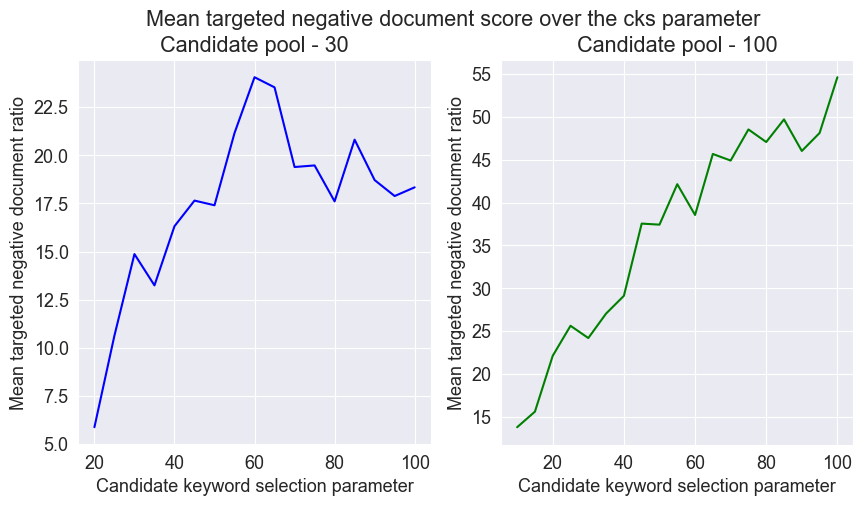
\includegraphics[width=.99\textwidth]{images/subplots/csk_tfn_score_subplot.png}
	\caption[Targeted negative document ratio over cks parameter.]{Targeted negative document ratio over candidate keyword selection parameter.  \label{fig:target_function_vs_csk}}
\end{figure}

\prettyref{fig:target_function_vs_csk} presents the relationship between the mean targeted negative document ratio and the $cks$ parameter. This metric indicates the separation of clusters based on their similarities. The results from the small candidate pool show the highest separation of negative documents at $cks$ = 60 and a downward trend for values of $cks$ higher than 60. This suggests that keyword selection has a positive impact on clustering, achieving better separation. In contrast, the results from the large candidate pool yield different outcomes. There is a clear upward trend, implying that no keyword selection (i.e., $cks$ = 100) has resulted in better separation of clusters. However, the results from the large candidate pool do not truly represent the nature of this evaluation metric, as it ignores the unlabeled documents after clustering. Considering the labels of all 100 documents may lead to different results.

\begin{center}
	\captionof{table}[Mean of evaluation metrics for CP-30.]{Mean of evaluation metrics over the cks parameter for the small candidate pool (30).}\label{tab:top_5_smallcdd}
	\begin{tabularx}{.8\textwidth}{|Y|Y|Y|Y|}
		\hline
		Objective function score &  Mean silhouette score &  Mean targeted negative document ratio &  Cks parameter \\
		\hline
		
		  \textbf{0.48}  &            0.42 &                         20.81 &      85   \\ \hline
		0.46 &            0.41 &                         19.48 &           75 \\ \hline
		0.45 &            0.39 &                         24.06 &           60 \\ \hline
		0.45 &            0.42 &                         18.34 &           100 \\ \hline
		0.45 &            0.42 &                         17.89 &           95 \\ \hline
		
	\end{tabularx}
	
\end{center}

\begin{figure}[h]
	\centering
	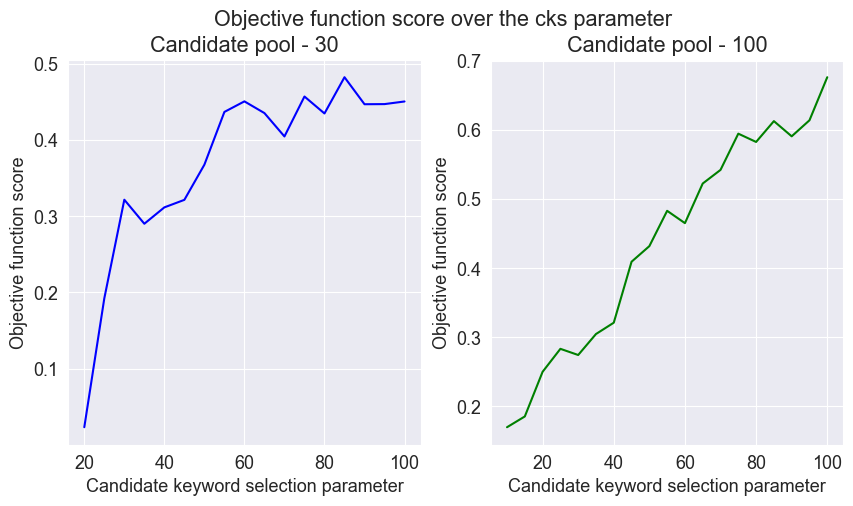
\includegraphics[width=.99\textwidth]{images/subplots/harmonic_score_cks_subplot.png}
	\caption[Objective function score analysis over cks parameter.]{Objective function score analysis over candidate keyword selection parameter. \label{fig:objective_function_vs_csk}}
\end{figure}

The analysis results from intrinsic and extrinsic measures have shown different patterns for the small candidate pool and similar patterns for the large candidate pool. Combining these two measures, a final objective function score, which is the harmonic mean of the normalized intrinsic and extrinsic measures, is calculated. \prettyref{fig:objective_function_vs_csk} presents the relationship between the objective function score and the $cks$ parameter. For the small candidate pool, the highest objective function score is achieved at a keywords selection of 85. This indicates that selecting keywords below the 85th percentile similarity generates better clustering.

However, it is important to note that the top 15 percentile keywords may only consist of around 3 to 4 keywords or even fewer. Therefore, the improvement in clustering between the $cks$ values of 85 and 100 is minimal. Additionally, the keyword selections at 60 and 75 also yield very close results compared to the highest score at 85. \prettyref{tab:top_5_smallcdd} presents the top 5 $cks$ parameter results ordered by the objective function score for the small candidate pool. Although the 85th percentile selection has the highest objective function score, there is no significant difference in the scores when compared to other percentile selections.

\begin{center}
	\captionof{table}[Mean of evaluation metrics for CP-100.]{Mean of evaluation metrics over the cks parameter for the large candidate pool (100)}.\label{tab:top_5_largecdd}
	\begin{tabularx}{.8\textwidth}{|Y|Y|Y|Y|}
		\hline
		Objective function score&  Mean silhouette score &  Mean targeted negative document ratio & Cks parameter   \\
		\hline
		
		\textbf{0.68} &            0.50 &                         54.62 &           100 \\ \hline
		0.61 &            0.49 &                         48.12 &           95 \\ \hline
		0.61 &            0.48 &                         49.70 &           85 \\ \hline
		0.59 &            0.48 &                         48.53 &           75 \\ \hline
		0.59 &            0.49 &                         46.02 &           90 \\ \hline
		
	\end{tabularx}
	
\end{center}

On the other hand, the large candidate pool shows an increase in the objective function score with a larger candidate keyword selection. \prettyref{tab:top_5_largecdd} presents the top 5 $cks$ parameter results ordered by the objective function score for the large candidate pool. These results clearly indicate that there is no benefit to keyword selection, as the $cks$ parameter value of 100 yields the highest evaluation scores.

\subsection{Missed Document Analysis}

The proposed methodology clusters keywords within a document rather than clustering the documents themselves. Documents are represented as a set of clustered keywords. This approach leads to a soft-clustering output, where a document can be assigned to multiple clusters if it contains keywords from different clusters. The clustering algorithm, \ac{HDBSCAN}, considers inherent noise in the data and does not assign all keywords to specific clusters. This results in the creation of noise keywords that do not belong to any cluster. If a document only contains keywords that are part of the noise keywords, it is missed (removed) during the modeling process. Analyzing the missed documents is crucial because if more documents are removed, the document modeling loses its significance.


\begin{center}
		\captionof{table}{Mean missed document values over the cks parameter.}\label{tab:mean_missed_documents}
	\begin{tabular}{ cc }   % top level tables, with 2 columns
		Candidate pool - 30 & Candidate pool - 100 \\  
		% leftmost table of the top level table
		\begin{tabularx}{.4\textwidth}{ |Y|Y| } 
			\hline
			Cks parameter & Mean missed documents  \\
			\hline
			20 & 0.94  \\
			\hline
			40 & 0.75  \\
			\hline
			60 & 0.40  \\
			\hline
			80 & 0.18  \\
			\hline
			100 & 0.09  \\
			\hline
		\end{tabularx} &  % starting rightmost sub table
		% table 2
		\begin{tabularx}{.4\textwidth}{ |Y|Y| } 
			\hline
			Cks parameter & Mean missed documents  \\
			\hline
			20 & 1.07  \\
			\hline
			40 & 0.59  \\
			\hline
			60 & 0.34  \\
			\hline
			80 & 0.11  \\
			\hline
			100 & 0.01  \\
			\hline
		\end{tabularx} \\
	\end{tabular}
\end{center}


 \prettyref{tab:mean_missed_documents} shows the average number of missed documents over the candidate selection parameter. This includes all possible combinations of the hyperparameter set and the queries from the test set. In the case of a small candidate pool, only one document, on average, is missed for lower values of the $cks$ parameter. It is important to note that the missed documents for certain queries may be higher than the average scores, as only the mean is considered here. For large $cks$ values, the average number of missed documents is very small, indicating minimal loss of documents during the subtopic modeling. A similar pattern is observed in the large candidate pool, where low values of the $cks$ parameter result in a higher loss of documents. This data suggests avoiding a candidate selection of less than the 40th percentile, as it can potentially lead to the loss of documents during the modeling process.

\subsection{Parameter Selection Analysis}


This section details the clustering performance for the top-5 parameters when considered individually. In the earlier analysis, the results are grouped over the candidate keyword selection ($cks$) parameter. \prettyref{tab:parameter_sel_small} details the hyperparameters and respective objective function scores for the small candidate pool. There is a huge variation in the "minimum samples" parameter among the top-5 results. This parameter implies the minimum number of data points in a cluster. A value of 1 signifies that a minimum of one data point can create a cluster. However, this would result in many clusters with very few data points, leading to poor clustering despite the evaluation metrics showing better performance. The change in the $cks$ parameter between the values 90, 95, and 100 will not have a significant impact on the clustering output, as the number of selected keywords lies within the 5th percentile, which can be very low.

\begin{center}
	\captionof{table}[Objective score analysis for CP-30.]{Objective score analysis over the parameters for the small candidate pool (30).}\label{tab:parameter_sel_small}
	\begin{tabularx}{.8\textwidth}{|Y|Y|Y|Y|Y|}
		\hline
		 Objective function score &  Reduced dimensions &  Minimum cluster size &  Minimum samples & Cks parameter \\
		\hline
		
		\textbf{ 0.896} &      10.0 &              20.0 &          1.0 &          100 \\		\hline
		\textbf{ 0.896}  &       5.0 &              20.0 &          7.0 &          95 \\		\hline
		0.878 &      10.0 &              20.0 &          3.0 &          100 \\		\hline
		0.848 &       5.0 &              20.0 &          1.0 &          90 \\		\hline
		0.848 &       5.0 &              20.0 &          5.0 &          95 \\		\hline
		
	\end{tabularx}
	
\end{center}



\begin{center}
	\captionof{table}[Objective score analysis for CP-100.]{Objective score analysis over the parameters for the large candidate pool (100).}\label{tab:parameter_sel_large}
	\begin{tabularx}{.8\textwidth}{|Y|Y|Y|Y|Y|}
		\hline
		 Objective function score &  Reduced dimensions &  Minimum cluster size &  Minimum samples & Cks parameter \\
		\hline
		
		\textbf{0.964} &       5.0 &              20.0 &         10.0 &          100 \\ \hline
		0.946 &      10.0 &              20.0 &         10.0 &          100 \\ \hline
		0.941 &      10.0 &              20.0 &          5.0 &          100 \\ \hline
		0.939 &      10.0 &              20.0 &          7.0 &          100 \\ \hline
		0.935 &       5.0 &              20.0 &          7.0 &          100 \\ \hline
		
	\end{tabularx}
	
\end{center}

Comparatively, the parameters such as reduced dimensions and minimum cluster size have very little variation. \prettyref{tab:parameter_sel_small} shares similar data for the large candidate pool. From this data, a higher minimum sample of 10 shows better clustering results, contrary to the small candidate pool. To generate a diverse clustering output, the cluster size should be relatively larger rather than very small clusters. Small clusters are generated when a minimum of one or three data points can be considered as noise clusters and are not desired. From both candidate pools, a minimum cluster size of 20 and a reduced dimension of 5 can be chosen for the final parameter selection. The final parameters selected after this analysis are shown in \prettyref{tab:ideal_parameters}.


\begin{center}
	\captionof{table}{Parameters selected after parameter selection analysis. }\label{tab:ideal_parameters}
	\begin{tabularx}{.4\textwidth}{|Y|c|}
		\hline
		   Parameter & Value\\
		\hline
		
	        Cks parameter &          100 \\ \hline
		       Reduced dimensions &          5 \\ \hline
         Minimum cluster size &          20 \\ \hline
	        Minimum samples &          10 \\ \hline
		
	\end{tabularx}
	
\end{center}


\subsection{Manual Interpretation of Results}

After selecting the parameters by observing the clustering performance for both the small and large candidate pools, a manual evaluation is performed on the large candidate pool. The clustering results provide deep insights into the candidate pool. However, it is also observed that the effectiveness of the selected parameters in generating heterogeneous clusters still needs to be improved (not achieved through automatic parameter selection). The main reason for the poor clustering results in terms of diversity is the absence of keyword selection, i.e., $cks$ = 100. Generating deep clusters while maintaining cluster uniqueness is a challenging task. Evaluation metrics need to be more successful in capturing this problem. Manual analysis is carried out on multiple clustering outputs using the parameters mentioned in \prettyref{tab:ideal_parameters} and different values of the $cks$ parameter.
 
 \begin{center}
 	\captionof{table}[Manual clustering output analysis.]{Manual clustering output analysis for the Query "5G" with different cks parameters. }\label{tab:5G_output}
 	\begin{tabularx}{.9\textwidth}{|c|c|Y|}
 		\hline
 		Cks parameter & Number of cluster & Sub-topics (clusters)\\
 		\hline
 		
 		100 &          34 & 5G, 5G network, Frequenzspektrum, 5G deployment, China, Defence intelligence, Nokia, Berlin, Mobilfunkmast, Telekom, Gigabit speed, 4G, WiFi, UMTS, Military, Fiberoptic broadband, 5G technology, Vodafone, Experimentation testing, Mobilfunknetzbetreiber, Technologie, Netzwerk, LTE, Smartphones, Netz, Aircraft, 5G service, Data cap, Deutsche Telekom, Telefónica, Apple, Gebiet, Netzausbau, Anbieter \\  \hline
 		 75 &          23 & Anstieg, TelekomKunden, Netzausbau, ATT, Mobilfunkmast, Military, Frequenzspektrum, Defense cybersecurity, Berlin, Nokia Ericsson, Experimentation testing, USA, Fiberoptic broadband, Smartphones, Technologie, 4G network, Carrier, Military aviation, ISP, WiFis reach, Upload speed, Apple, 5G telecommunication \\ \hline
 		50 &          14 & Deutschland, Fortschritt, Telecom, Mobilfunkantenn, Wireless ISPs, Frequenzspektrum, 4G network, Military, Defense cybersecurity, Technologie, Netzausbau, Nokia Ericsson, Experimentation testing, Military aviation \\  \hline
 		25 &          10 & Ausbau, Military aviation, Testing experimentation, Trump administration, Verizon wireless, SmartphoneNutzer, Telekommunikationsdienstleister, Berliner Hauptbahnhof, Frequenzspektrum, Technologieführerschaft \\  \hline
 		
 	\end{tabularx}
  \end{center}
 
 
The results of one query, namely "5G," are presented in \prettyref{tab:5G_output}. The subtopics generated when no keywords are selected are highly redundant and may not be useful to the users, as they have less significance. For example, the subtopics "5G" and "5G network" are very similar and might lead to the same set of documents. The objective of creating unique pathways from the user query to retrieved documents is not achieved. The clustering output using the 75th percentile similarity selection shows a similar clustering result. The practicality of subtopics in the real world is only successful when the clusters are unique and diverse. On the other hand, the clustering outputs for the $cks$ parameters of 25 and 50 are unique, as we have removed a significant amount of keywords similar to the query. However, there is a high chance of missing documents in this scenario.
 
 
 \begin{center}
 	\captionof{table}[Results from manual cks parameter selection of 65.]{Results from manual cks parameter selection of 65 for different queries. }\label{tab:65_output}
 	\begin{tabularx}{.9\textwidth}{|c|c|Y|}
 		\hline
 		Query & Number of cluster & Sub-topics (clusters)\\
 		\hline
 		
 		5G  &          18 & 5G telecommunication, 4G network, Broadband, ATT Verizon, WiFis reach, Smartphone, Frequenzspektrum, Netzausbau, Fortschritt, Mobilfunkmast, Deutschland, Carrier, Telekommunikationskonzer, Experimentation testing, Technologie, Defense cybersecurity, Aircraft, Military \\  \hline
 		
 		Quantentechnologie &          23 & Industriebetrieb, Quantum physic, DAQC, SuperRechner, Vorsprung, Datennetzwerk, Luft Raumfahrt, Forscher, Simulation, AI, Qubit, IBM, Datum, Department defense, AmazonGründer, Deutschland, Entwicklung, Military, Congress, Marineschiffbau, Forschung, Bundesministerium, China \\  \hline
 		
 	\end{tabularx}
 
  \end{center}


\prettyref{fig:target_function_vs_csk} shows a downward trend in the targeted negative document ratio at $cks$ = 60 for the small candidate pool. This signifies that there is better separation between the clusters at $cks$ = 60, and then it decreases for higher $cks$ values. However, only the larger candidate pool results are analyzed manually, rather than the small candidate pool. Despite this difference, the information from the small candidate pool can be partly helpful, as it uses the labeled information. Therefore, a 65th percentile similarity selection is chosen after a manual analysis of several queries. The results of the manual parameter selection with $cks$ = 65 are shared in \prettyref{tab:65_output}. There are still some redundant clusters at this selection, but the results are better than with higher selection values. The choice of this particular 65th percentile selection is not only due to the heterogeneity of clusters but also to minimize the loss of documents during clustering. Similarly, an 85th percentile selection is chosen for the smaller candidate pool. The final parameters through the manual selection are presented in \prettyref{tab:manual_parameter_selection}. Furthermore, the results from the 65th percentile selection are evaluated during the survey feedback and will be shared in upcoming sections.
 
 \begin{center}
 	\captionof{table}{Final parameters selected after manual analysis.}\label{tab:manual_parameter_selection}
 	\begin{tabularx}{.5\textwidth}{|Y|c|c|}
 		\hline
 		Parameter & CP-30 & CP-100 \\
 		\hline
 		
 		Cks parameter & \textbf{85} &         \textbf{65} \\ \hline
 		Reduced dimensions &  5  &       5 \\ \hline
 		Minimum cluster size & 20 &         20 \\ \hline
 		Minimum samples &    10  &     10 \\ \hline
 		
 	\end{tabularx}
 	
 \end{center}
 
 \subsection{Ineffectiveness of Target Functions}
 
The manual parameter selection has shown great results by generating a diverse set of sub-topics, as observed in \prettyref{tab:5G_output} and \prettyref{tab:65_output}. Silhouette score and targeted negative document ratio are used to automatically select parameters. However, the target functions are not very successful in capturing the patterns that distinguish clusters. One crucial reason for this outcome is the lack of sub-topic labels. The test set used in this master thesis contains labels at the document level, meaning that a document is labeled as either relevant or irrelevant for a given query. There are no ground-truth labels for the sub-topic clustering output. Other reasons for the ineffectiveness of target functions are highlighted below.
 
 \begin{description}
 	\item[Silhouette score]  \hfill \\ 
Silhouette score evaluates the quality of clustering output by calculating the point-wise distance between the data points inside and outside its cluster. It is generally used to select the number of clusters for a dataset. The aspect of distinctiveness of clusters deals with the semantic nature of the cluster labels. The results from \prettyref{fig:silhouette_score_vs_csk} show that the distinctiveness of clusters is not related to the quality of clusters calculated with distance metrics. Therefore, due to the lack of consideration for the semantic nature of the expected output, silhouette score tuning has not generated diverse sub-topic results.
 	
 	\item[Targeted negagive document ratio]  \hfill \\ 
This target function calculates the quality of separation of documents based on the document labels. It divides the clusters into either positive or negative clusters. Clusters with a relatively high number of positive documents (labeled as either perfect or partially relevant) are considered as the positive clusters, and the rest are negative clusters. \prettyref{fig:target_function_vs_csk} shows that this target function is effective in the case of a small candidate pool at $cks$ = 60 and has no significance in a large candidate pool. One main reason for this pattern is the availability of labeled documents in small and large candidate pools, as all documents in large candidate pools are labeled.
 	
 The test has very few positive documents for most of the queries, which results in fewer positive clusters and more negative clusters. In addition to that, the definition of negative clusters is not precisely defined and considered as the negation of positive clusters. It is also observed that the $cks$ parameter has no direct influence on the creation of positive clusters. The clustering output is directly dependent on the keywords extracted from the documents, and the separation of clusters is dependent on the document labels.
 	
 	
 	
 \end{description}
 
 	
\subsection{Key Statistics from Clustering}

After finalizing the parameters from \prettyref{tab:manual_parameter_selection} with a 65th percentile selection for the large candidate pool and an 85th percentile selection for the small candidate pool, an analysis is carried out on the cluster metadata. Three clustering observations are collected from the sub-topic modeling and presented in ~\prettyref{tab:keyword_analysis}. All the data presented below are calculated over 17 queries in the test set.

\begin{enumerate}
	\item \textbf{Mean number of clusters} gives the average number of clusters/sub-topics after sub-topic modeling.
	\item \textbf{Mean keywords size} gives the average number of keywords used during the sub-topic modeling.
	\item \textbf{Mean cluster size} gives the average number of keywords per cluster.
\end{enumerate}

\begin{center}
	\captionof{table}{Keyword observations during clustering over 17 queries.}\label{tab:keyword_analysis}
	\begin{tabularx}{.6\textwidth}{|Y|c|c|}
		\hline
		Parameter & CP-30 & CP-100 \\
		\hline
		Mean number of clusters & 7.06 & 19.41 \\
		\hline
		Mean keywords size & 423.59 & 1057.47 \\
		\hline
		Mean cluster size & 70.12 & 78.96 \\
		\hline
	\end{tabularx}
\end{center}

It is evident from the above table that the large candidate pool considers more data points for clustering and generates around three times more sub-topics compared to the small candidate pool. This signifies that the user has the opportunity to view more diverse sub-topics and can access more documents. The average cluster size remains almost the same in both candidate pools and signifies that clustering parameters are well selected.

 \subsection{Document Repetition Analysis}
 
The proposed approach in this master thesis assigns a news article to multiple clusters according to their keyword information. This approach can lead to poor modeling of documents when several documents appear in many clusters. There is a possibility of users getting annoyed by reading the same documents in multiple clusters. Therefore, a high document repetition in clusters is considered poor modeling. To evaluate this scenario in the case of the proposed candidate keyword selection approach, an evaluation metric, namely \textit{\ac{MCC}}, is proposed. The cluster count of a document $CC_d$ is calculated as the number of clusters that contain the document $d$. The query cluster count of a query $QCC_q$ is calculated as the mean of cluster counts over all documents $J$ clustered for the query $q$. Similarly, \ac{MCC} is calculated as the mean of $QCC_q$ over all $N$ queries in the test set.

\centerline{$QCC_q$ = ($\sum\limits_{i=1}^J CC_i) /J$}
\centerline{$MCC$ = ($\sum\limits_{i=1}^N QCC_i) /N$}

\prettyref{tab:mean_cluster_count} shows the mean cluster count information over four $cks$ percentile selections. The data is compared against the mean number of clusters information shared in~\prettyref{tab:keyword_analysis}. In the case of CP-30 and $cks$ = 100, the \ac{MCC} is 4.35, which signifies that, on average, a document is present in over four clusters. The average number of clusters for CP-30 is around 7. This implies that, on average, a document is present in more than half of the clusters, and the user encounters the same document again and again. This can lead to poor usability of the sub-topic retrieval approach. On the other hand, when the $cks$ = 50 in CP-30, the \ac{MCC} is around 2, indicating that a document repeats in two clusters, which is relatively lower than the average number of clusters. Therefore, the $cks$ parameter has a significant impact on effectively modeling documents and can possibly improve the usability of the retrieval.

\begin{center}
	\captionof{table}{Mean cluster count over cks percentile parameter. }\label{tab:mean_cluster_count}
	\begin{tabular}{ cc }   % top level tables, with 2 columns
		Candidate pool - 30 & Candidate pool - 100 \\  
		% leftmost table of the top level table
	\begin{tabularx}{.35\textwidth}{|Y|c|}
		\hline
		Cks parameter  & CP-30 \\
		\hline
		100 & 4.35  \\
		\hline
		75 & 2.93 \\
		\hline
		50 & \textit{2.23} \\
		\hline
		25 & 1.46 \\
		\hline
	\end{tabularx}&  % starting rightmost sub table
		% table 2
		\begin{tabularx}{.35\textwidth}{|Y|c|}
			\hline
			Cks parameter & CP-100 \\
			\hline
			100 & \textbf{6.63}  \\
			\hline
			75 & 5.31 \\
			\hline
			50 & 3.51 \\
			\hline
			25 & 2.01 \\
			\hline
		\end{tabularx}\\
	\end{tabular}
\end{center}

This pattern observed in CP-30 does not hold true for the large candidate pool. From~\prettyref{tab:keyword_analysis}, the mean number of clusters in the large candidate pool is around 19. In the case of CP-100 and $cks$ = 100, the \ac{MCC} is 6.63, which signifies that, on average, a document is present in around seven clusters. The \ac{MCC} value for $csk$ = 100 is very low compared to the mean number of clusters, i.e., 19. As the sub-topic count is relatively high, the impact of repeating documents is minimal for the users. Nevertheless, there is a high possibility of users reading the same document again from different clusters.



\section{Survey Results Evaluation}

The survey aims to evaluate the clustering output and the effectiveness of subtopics in finding relevant documents. A survey questionnaire with two unique retrieval systems and five questions is developed and evaluated by taking feedback from real users. The retrieval systems used in the survey use not only the query but also the sub-topic. The comparison is made to observe the system that represents both user inputs efficiently. A template, namely \textit{"Innovation in~\textbf{Query} and~\textbf{Sub-topic}"}, is used in both approaches to either retrieve or rerank the news articles. A brief description of retrieval systems A and B is shared below.

\begin{description}
	\item[System A] Retrieve new-articles using the sub-topic clustering output and then re-rank the retrieved results using template similarity.
	
	\item[System B] Retrieve new-articles using the template as a query and re-rank the results using template similarity.
\end{description}

The results from the survey directly answer the practicality of the proposed approach in this master's thesis. Participants must answer the questions according to the inputs provided through the user interface. The survey can be partially answered depending on the user's interest, resulting in an unequal number of participants for each question (as detailed in Section 6.5). \prettyref{tab:question_summarization} summarizes the questions asked in the survey.


\begin{center}
	\captionof{table}{Summarized description of the questions asked in the survey.}\label{tab:question_summarization}
	\begin{tabularx}{.8\textwidth}{|c|Y|}
		\hline
		Question id  & Summarized description \\
		\hline
		Question 1 & Is the sub-topic clustering output is distinctive and well-labeled?  \\
		\hline
		Question 2 & Which system better represents the user query and the sub-topic? \\
		\hline
		Question 3 & Rate the system A retrieval results (0-10) \\
		\hline
		Question 4 & Rate the system B retrieval results (0-10) \\
		\hline
		Question 5 &  Does the sub-topics helpful to retrieve relevant documents?\\
		\hline
	\end{tabularx}
\end{center}

The number of participants in each question is calculated by the unique UUID recorded during the session. One drawback of this approach is the need to recognize the same user performing in a different session. Due to privacy reasons, it is obligatory not to record the user details, and therefore a session-based approach is adopted here. Furthermore, multiple answers are expected from each participant. Accordingly, the number of user feedback inputs is higher than the participant count. The participant count score is shared in \prettyref{tab:participant_cnts}. Only a large candidate pool of around 100 documents is considered in the survey. In this section, only the survey results are shared, and the detailed survey questionnaire is accessible in Section 6.5.

\begin{center}
	\captionof{table}{Pariticpant counts in the survey.}\label{tab:participant_cnts}
	\begin{tabularx}{.6\textwidth}{|Y|c|}
		\hline
		Question id & Participant count \\
		\hline
		Question 1 & 12 \\
		\hline
		Question 2, 3, 4 & 8 \\
		\hline
		Question 5 & 8 \\
		\hline
	\end{tabularx}
\end{center}

\subsection{Subtopic Clustering Response Analysis}

The participants are asked to share feedback on the clustering results in this question. The quality of clusters is evaluated using the distinctiveness and readability of clusters. The results from the survey for this question are shared in \prettyref{fig:question_1_piechart}. The majority of the participants, around 44 percent, agree that the retrieved sub-topics are \textit{distinctive and not well-labeled}. Moreover, only 6 percent of the participants admit that the retrieved sub-topics are \textit{not distinctive and well-labeled}.

\begin{figure}[h]
	\centering
	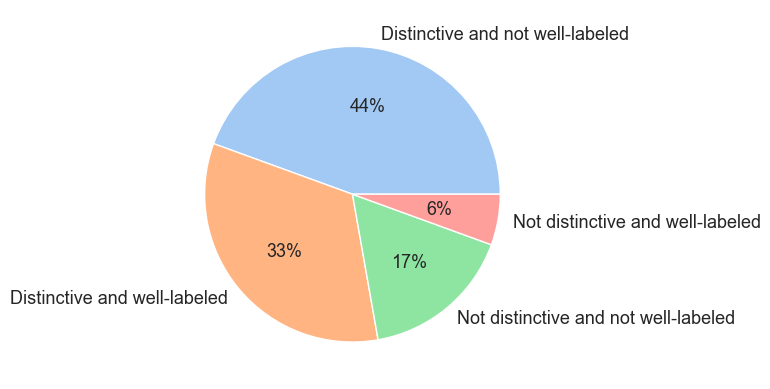
\includegraphics[width=.8\textwidth]{images/subplots/rating_piecharts.png}
	\caption[Sub-topic clustering output feedback.]{Piechart detailing the feedback on the sub-topic clustering output. \label{fig:question_1_piechart}}
\end{figure}

The user feedback is further analyzed individually and shared in \prettyref{fig:question_1_barplot}. Fourteen survey inputs agree with the distinctiveness of the sub-topics, and four inputs share contrary feedback, i.e., non-distinctive. Similarly, 11 user inputs show that the cluster labels or sub-topic names need to be better labeled, and seven inputs show the opposite pattern.

\begin{figure}[h]
	\centering
	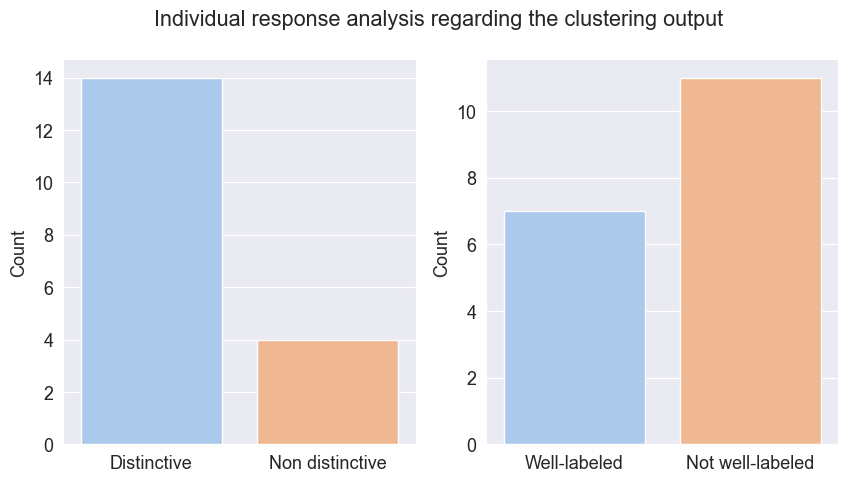
\includegraphics[width=.9\textwidth]{images/subplots/barplots.png}
	\caption{Barplot highlighting the individual response.  \label{fig:question_1_barplot}}
\end{figure}


It is evident from the above table that most of the survey participants agree with the distinctiveness of the sub-topics. Therefore, the candidate keyword selection positively impacts the clustering by creating distinctive clusters. However, the sub-topic labeling approach that uses the clusters' centroid needs to generate better results. After analyzing the sub-topic labels from \prettyref{tab:65_output} and \prettyref{tab:5G_output}, it can be observed that some of the sub-topics have abbreviations as labels. For example, DAQC, ATT, UMTS, etc., are some labels that might not be familiar to many participants and can lead to poor interpretation of the cluster and its documents.

\subsection{System Comparison Response Analysis}

These questions are targeted to evaluate the two IR systems developed to represent the retrieved documents. System A retrieves news articles using the sub-topic modeling output and re-ranks them using a dynamic template, while System B retrieves news articles with a new query request to the semantic index using the same template. Furthermore, quantitative ratings ranging from 0 to 10 are collected for both systems. Some participants have provided false inputs, and these inputs are considered anomalies. These anomaly feedback inputs for questions 2, 3, and 4 are removed from the analysis. One such feedback is observed and shared in \prettyref{tab:question_234_anamoly}. It is clear that the user has provided a lower rating for System B than for System A. However, the user has chosen System B as the better system, which clearly contradicts the individual ratings.


 \begin{center}
	\captionof{table}{Improper user feedback input in the survey. }\label{tab:question_234_anamoly}
	\begin{tabularx}{.8\textwidth}{|Y|c|c|}
		\hline
		Which IR system is better? & System A ratings & System B ratings \\
		\hline
		System B & 10 & 6.1 \\
		\hline
	\end{tabularx}
\end{center} 

Participants are requested to answer a qualitative comparison between the two systems, and the results are shared in \prettyref{tab:question_2_results}. After removing the anomalies, it is evident from \prettyref{tab:question_2_results} that most participants have agreed that 'System A' retrieves documents better than 'System B'. This result is derived from the qualitative inputs of the survey. However, it is crucial to determine the significance of this result through the quantitative inputs, i.e., system ratings.

\begin{center}
	\captionof{table}{Question 2, 3, and 4 results.}\label{tab:question_2_results}
	\begin{tabular}{ cc }   % top level tables, with 2 columns
		IR system comparison  & Questions 3 and 4 \\  
		% leftmost table of the top level table
\begin{tabularx}{.4\textwidth}{|Y|c|}
	\hline
	Label & Count \\
	\hline
	System A & 18 \\
	\hline
	System B & 0 \\
	\hline
	Neither System A nor System B & 4 \\
	\hline
	
\end{tabularx} &  % starting rightmost sub table
		% table 2
		\begin{tabularx}{.45\textwidth}{|c|c|Y|Y|}
			\hline
			System & Mean & Standard deviation & Variance \\
			\hline
			 A & 5.46 & 2.92  & 8.54 \\
			\hline
			 B & 3.28 & 2.77 & 7.7 \\
			\hline

		\end{tabularx} \\
	\end{tabular}
\end{center}

\prettyref{tab:question_2_results} shows that 'System A' has a better mean than 'System B', and there is no significant difference in the standard deviation. Individual system ratings are plotted in a histogram and presented in \prettyref{fig:histograms}. These distributions clearly show that 'System B' ratings are more concentrated towards lower values and follow a right-skewed distribution. On the other hand, 'System A' ratings are not concentrated at a certain level but rather follow a positive trend with some high ratings.

\begin{figure}[h]
	\centering
	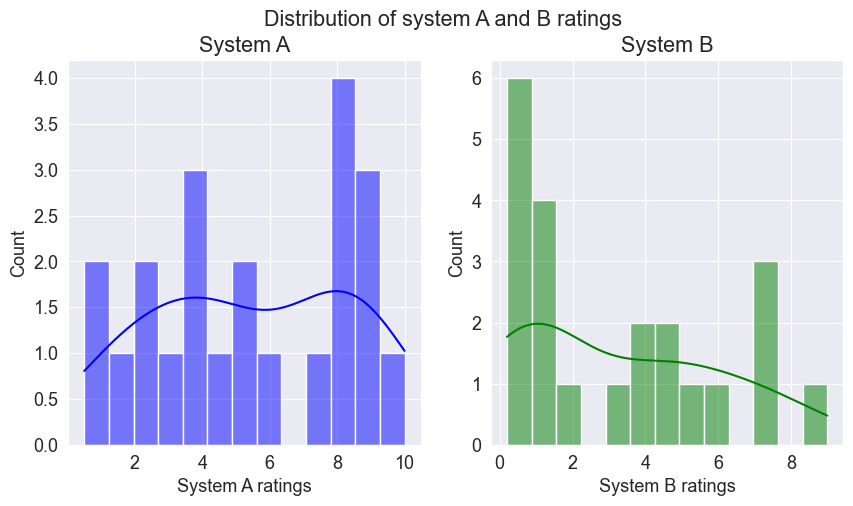
\includegraphics[width=.99\textwidth]{images/subplots/rating_histograms.png}
	\caption{Histograms showing the distribution of system ratings.  \label{fig:histograms}}
\end{figure}



The significance of one system performing better than the other can be evaluated with the help of statistical testing. The system ratings are collected for two systems for a given query and sub-topic. Therefore, the sample data can be considered as paired data as they are relative to each other and not compared with other queries or sub-topics. This relation between the data is also referred to as dependent data samples. \prettyref{fig:histograms} shows that the system ratings do not follow any specific distributions, and therefore, parametric statistical tests are not feasible. A non-parametric hypothesis test, namely the Wilcoxon signed-rank test~\cite{buWilcoxonSigned}, is chosen in this master's thesis. This statistical test considers the signs of the difference scores between the dependent data along with the magnitude of the differences. In the Wilcoxon Signed Rank Test, the hypothesis is built on the median of the difference scores~\cite{buWilcoxonSigned, kaur2015comparative}.


\begin{enumerate}
	\item \textbf{Null Hypothesis ($H_0$)}: The median difference between the samples, namely "System A" and "System B" ratings is zero.
	
	\item \textbf{Alternate Hypothesis ($H_1$)}:  The median difference between the samples, namely "System A" and "System B" ratings is not zero.
\end{enumerate}

The hypothesis is based on whether the median difference is equal to zero or not, rather than being compared to a specific value. Thus, this is referred to as a two-tailed test. Before performing the statistical testing, it is crucial to choose the confidence level and the test statistic. A confidence level of 95\% is chosen, i.e., a significance level ($\alpha$) of 0.05, and for the test statistic, the z-score is selected. \prettyref{fig:z_score} shows the acceptance and rejection regions for the significance level $\alpha$ = 0.05. If the test score is lower than -1.96 or greater than 1.96, the null hypothesis should be rejected, and the alternative hypothesis should be accepted. In any other case, the null hypothesis must be accepted.


\begin{figure}[h]
	\centering
	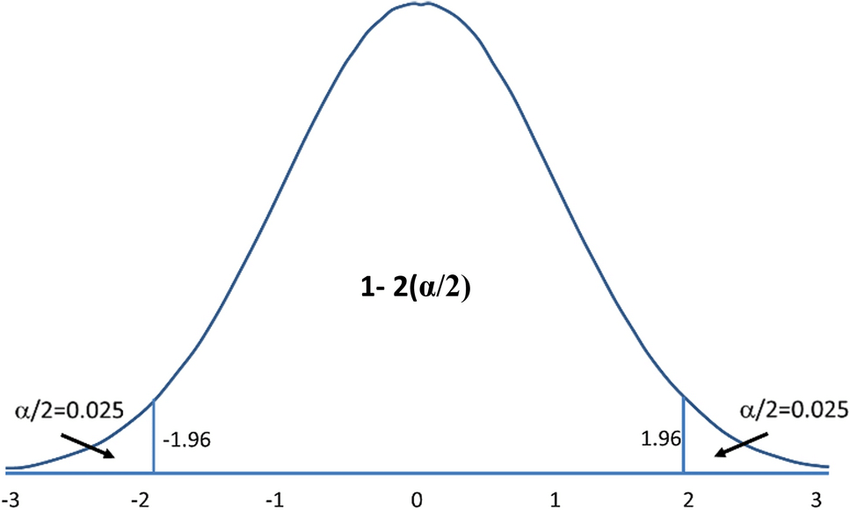
\includegraphics[width=.75\textwidth]{images/outside/z_score.PNG}
	\caption[Rejection regions for z test-statistic.]{Rejection regions for a significance level of 0.05 and z test-statistic. \cite{article} \label{fig:z_score}}
\end{figure}



The test statistic is calculated using the python library \textit{researchpy}\footnote{\url{https://researchpy.readthedocs.io/en/latest/index.html}}. The calculated z-score is 4.06, and the test score is larger than the critical value of 1.96. Therefore, the null hypothesis is rejected, and the alternative hypothesis is accepted. This means that the system ratings are significantly different, and System A retrieves better news articles related to the user query and the sub-topic. This concludes the system comparison by suggesting that retrieval using the sub-topic modeling output has performed better than a new query request.

\subsection{System Comparison Query Analysis}

The system comparison is statistically evaluated, with the conclusion that System A represents the news articles better based on the sub-topic clustering output. However, the mean system A ratings from the participants are around 5.46, which is not high on a scale of 10. From \prettyref{fig:histograms}, it is evident that a few responses for System A are high, while the other ratings are very low. To understand the user responses, the high and low ratings of System A are analyzed. The query and sub-topics used for System A are presented in \prettyref{tab:queries_question_234}.

\begin{center}
	\captionof{table}{Query and sub-topic analysis for system A. }\label{tab:queries_question_234}
	\begin{tabular}{ cc }   % top level tables, with 2 columns
		Top-25 percentile ratings & Bottom-25 percentile ratings \\  
		% leftmost table of the top level table
		\begin{tabularx}{.4\textwidth}{|Y|Y|}
			\hline
			Query  & Sub-topic \\
			\hline
			Künstliche Intelligenz & KI  \\
			\hline
			Künstliche Intelligenz & Military \\
			\hline
			Kryptographie & \textbf{Polizei Geheimdienst}\\
			\hline
			china Image recognition & Privacy \\
			\hline
		\end{tabularx}&  % starting rightmost sub table
		% table 2
		\begin{tabularx}{.55\textwidth}{|Y|c|}
			\hline
			Query  & Sub-topic \\
			\hline
			Main Ground Combat System & \textbf{Projekt}  \\
			\hline
			Main Ground Combat System & Laser beam \\
			\hline
			Edge computing & \textbf{SOSA} \\
			\hline
			Edge computing & Everbetter processor \\
			\hline
			Geoinformationen & \textbf{Operationsführung} \\
			\hline
			Semantische Technologien & \textbf{March} \\
			\hline
		\end{tabularx}\\
	\end{tabular}
\end{center}

From the bottom 25 System A ratings, it can be observed that the sub-topics chosen for retrieving news articles are unusual and not well related to the query. For example, the sub-topic \textit{Projekt} is too generic for a military query keyword such as \textit{Main Ground Combat System}. Similarly, the sub-topics \textit{March, SOSA, Operationsführung} lead to poor results as they do not effectively represent the sub-topic clusters. This pattern aligns with earlier observations where the majority of participants chose 'Not well-labeled' for the sub-topics. The sub-topic labeling is created using a centroid-based approach, which assigns the keyword closest to the centroid as the label of the cluster, disregarding key criteria such as abbreviations, understandability, uniqueness, etc.

\subsection{Subtopic Retrieval Response Analysis}

Participants are requested to share feedback on finding relevant documents using the proposed approach. The actual question asked in the survey is "Were the sub-topics helpful for you to find the relevant documents?". There are only two options to answer this question: 'Yes' or 'No'. The results show that around half of the participants found that the approach of retrieving documents using sub-topics does not help find news articles related to innovation.

\mycomment{One drawback of this question is that it does not specify
	the particular IR system. This can lead the users to provide biased input during the survey.
	To overcome this, two questions specific to two systems (A and B) should have been asked to the
	participants.}


\begin{center}
	\captionof{table}{Question 5 results.}\label{tab:question_5_results}
	\begin{tabularx}{.3\textwidth}{|Y|c|}
		\hline
		Label & Count \\
		\hline
		Yes & 6 \\
		\hline
		No & 5 \\
		\hline
	\end{tabularx}
\end{center} 

One reason for this could be the lack of relevant documents in the database for a particular query and sub-topic. Another reason could be the need for participants to assess the relevance of the retrieved documents, as the expected number of relevant documents might be low. Assuming these cases are different from the ones observed here, the proposed approach did not successfully assist the users in finding the relevant documents. On the other hand, participants who found it helpful suggest the possibility of using this approach to find relevant documents.

\subsection{Subtopic Retrieval Query Analysis}

The user queries collected for the sub-topic retrieval question are analyzed and shown in \prettyref{tab:queries_question_5}. The queries are divided into two categories: 'Yes' or 'No', based on the participants' responses. It is observed that the participants have provided positive feedback for search queries related to \textit{Technology}. On the other hand, there are only two queries related to \textit{Military}, such as \textit{Main Ground Combat System} and \textit{Geoinformationen}, and they have received negative feedback. This indicates that the users are not satisfied with the retrieved results for military-related queries.

\begin{center}
	\captionof{table}{Queries collected for the subtopic retrieval effectiveness.}\label{tab:queries_question_5}
	\begin{tabularx}{.8\textwidth}{|Y|Y|}
		\hline
		Yes & No \\
		\hline
		Künstliche Intelligenz  & \textbf{Main Ground Combat System} \\
		\hline
		Mobile Kommunikation & \textbf{Geoinformationen} \\
		\hline
		Quantentechnologie & \textbf{Edge computing} \\
		\hline
		Kryptographie & \textbf{Semantische Technologien} \\
		\hline
		china Image recognition & Robotik \\
		\hline
	\end{tabularx}
\end{center} 

One possible reason for the queries receiving negative feedback is the sub-topic selected by the participants. This can be observed from \prettyref{tab:queries_question_234} for the queries \textit{Edge computing} and \textit{Semantische Technologien}. However, the sub-topic information is not collected during the assessment of sub-topic retrieval effectiveness. Therefore, it cannot be determined whether the choice of sub-topic is the reason for the poor retrieved results.


\section{Precision Analysis Results}

This section details the results of the exploratory analysis on the ranking of sub-topics and the documents within those sub-topics. These rankings aim to generate a unique series of retrieved documents that simulate the user's real-time traversal. The description of the IR systems developed in this master thesis is shared in Section 6.6 and briefly presented again in \prettyref{tab:ir_system_intro}. Two evaluation metrics, namely mean expectation score and mean average precision, are used to evaluate the ranking output. Only a small candidate pool (CP-30) is used for this analysis, as labeled data is required to calculate the mean expectation and precision scores.


\begin{center}
	\captionof{table}{Brief IR system introduction.}\label{tab:ir_system_intro}
	\begin{tabularx}{0.8\textwidth}{|c|Y|Y|}
		\hline
		IR system name & Sub-topic ranking & Document ranking \\
		\hline
		IR0 & NA & Uniform distribution  \\
		\hline
		IR1 & NA & Query similarity \\
		\hline
		IR2 & Query similarity & Query similarity \\
		\hline
		IR3 & Template similarity & Template similarity \\
		\hline
		IR4 & Document cardinality & Query similarity \\
		\hline
		IR5 & (IR4, IR2) &  Query similarity \\
		\hline
		IR6 & (IR4, IR2, IR3) & Query similarity \\
		\hline
		IR7 & Random combinations & Query similarity  \\
		\hline
	\end{tabularx}
\end{center}

\subsection{Mean Expectation Score Analysis}

Expectation scores are calculated at a specific index, indicating the number of relevant documents. This analysis utilizes the mean expectation score, averaged over the 17 queries in the test set. For instance, a mean expectation score ($ME_5$) of 2 at index 5 signifies that, on average, there are two relevant documents among the top 20 retrieved documents. The higher the mean expectation score of an IR system, the better the retrieval performance. This analysis is crucial for users interested in reading documents at a specific index, allowing them to choose the best IR system accordingly.

\begin{figure}[h]
	\centering
	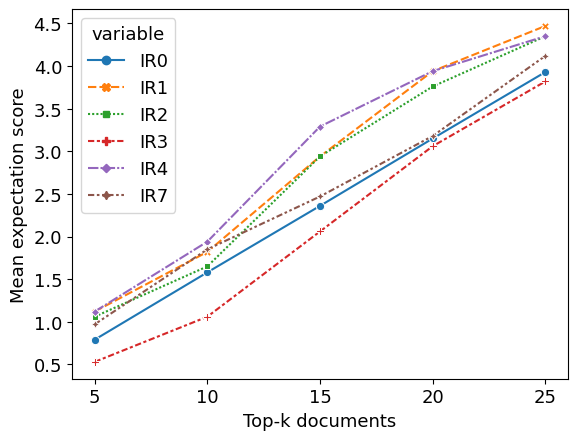
\includegraphics[width=.85\textwidth]{images/subplots/mean_expectation_score.png}
	\caption{Mean expectation score plot. \label{fig:mae_fig}}
\end{figure}

\prettyref{fig:mae_fig} presents the mean expectation score of six IR systems across five retrieval indices. Combinational IR systems, namely IR5 and TR6, are excluded from this plot as their results were similar to IR4 and thus redundant. One notable observation from \prettyref{fig:mae_fig} is that the IR4 system, which employs template similarity, performs poorly compared to the other IR systems. The same retrieval technique is used in the survey. The remaining IR systems exhibit similar patterns and are closely related. At index 15, the IR4 system, utilizing document cardinality, demonstrates relatively better performance than the other retrieval systems.


\begin{center}
	\captionof{table}{Mean expectation score results.}\label{tab:mae_results}
	\begin{tabularx}{0.8\textwidth}{|Y|c|c|c|c|c|}
		\hline
		IR system name & ME@5 & ME@10 & ME@15 & ME@20 & ME@25 \\
\hline
IR0 &          0.79 &           1.58 &           2.36 &           3.15 &           3.93 \\ \hline 
IR1 &          \textbf{1.12} &           1.82 &           2.94 &          \textbf{3.94} &           \textbf{4.47} \\ \hline
IR2 &          1.06 &           1.65 &           2.94 &           3.76 &           4.35 \\ \hline
IR3 &          0.53 &           1.06 &           2.06 &           3.06 &           3.82 \\ \hline
IR4 &           \textbf{1.12}  &            \textbf{1.94}  &          \textbf{3.29} &           \textbf{3.94} &           4.35 \\ \hline
IR5 &           \textbf{1.12}  &           \textbf{1.94} &           \textbf{3.29} &       \textbf{3.94}&           4.41 \\ \hline
IR6 &          \textbf{1.12}  &           \textbf{1.94} &           \textbf{3.29} &           3.88 &           4.41 \\ \hline
IR7 &          0.97 &           1.85 &           2.47 &           3.18 &           4.12 \\ \hline
	\end{tabularx}
\end{center}

\prettyref{tab:mae_results} displays the detailed expectation scores of the IR systems. Among the baseline systems, IR1, which does not utilize clustering, performed the best at the 25th retrieval index. However, the other IR systems, including IR7, which employs random combinations, exhibited better performance compared to the baseline systems IR0 and IR1. This clearly indicates that sub-topic clustering does not deteriorate the order of relevant documents as the user traverses through the sub-topics. Additionally, users benefit from the ability to select a specific sub-topic and directly access the relevant documents, enhancing retrieval efficiency.

\subsection{Mean Average Precision Analysis}

Mean average precision (MAP) provides a concrete score for comparing different IR systems based on the retrieved documents. Without specific index analysis, the IR system with the highest MAP score can be identified as the best IR system. \prettyref{tab:map_results} presents the MAP scores of the IR systems. Similar to the mean expectation scores, the IR3 system, which employs template similarity, performs poorly compared to other systems. Despite having the highest MAP score, the combination systems IR5 and IR6 do not demonstrate any improvement in retrieval performance. Combining multiple sub-topic rankings to generate a unified document ranking could yield more successful results, with one main reason being the need for a greater count of relevant documents.


\begin{center}
	\captionof{table}{Mean average precision results.}\label{tab:map_results}
		\begin{tabularx}{0.4\textwidth}{|c|Y|}
		\hline
		IR system name & MAP \\
		\hline
		IR0 & 0.185 \\
		\hline
		IR1 &  0.3 \\
		\hline
		IR2 &  0.303 \\
		\hline
		IR3 &  0.198 \\
		\hline
		IR4 &   \textbf{0.316} \\
		\hline
		IR5 &    \textbf{0.316} \\
		\hline
		IR6 &   0.315\\
		\hline
		IR7 &  0.292 \\
		\hline
	\end{tabularx}
\end{center}


The IR7 system, utilizing random combinations of sub-topic clusters, achieves a significant score and performs better than the baseline IR0. A simple document ranking based on query similarity without sub-topics (i.e., IR1) performs similarly to the IR2 system, which incorporates sub-topic ranking. This indicates that the retrieval performance remains consistent even with the introduction of sub-topics. Furthermore, the IR4 system, which utilizes document cardinality as the ranking criterion, performs the best. Although the difference is not significantly higher than other systems, IR4 possesses an inherent advantage over the baselines IR0 and IR1 in terms of accessing documents within a specific sub-topic.

\subsection{Ineffectiveness of Combinational IR systems}

Combinational IR systems, namely IR5 and IR6, have shown no significant improvement in performance. From the analysis results in \prettyref{tab:mae_results} and \prettyref{tab:map_results}, the combinational systems perform equally well or lower compared to the individual systems, such as IR4, which is based on document cardinality. The poor performance is due to the ineffectiveness of the algorithm in ranking positive documents at the top of the retrieved results. Retrieval performance is directly dependent on document ranking, which can be observed through MAP or MAE. These metrics are also greatly influenced by the number of positive documents, and it has been observed that the number of positive documents in the test set is relatively low.

Nevertheless, the effectiveness of the algorithm in generating combinational IR systems is evaluated by finding the unique document list generated through retrieval. To perform this analysis, two metrics are proposed: $R_s$, the number of unique sub-topic rankings, and $R_d$, the number of unique document rankings. Here, a unique ranking refers to a document or sub-topic ranking that differs from the rankings generated by the IR4 system. Generating new sub-topic and document rankings does not necessarily indicate better retrieval performance. However, it can reveal the effectiveness of the algorithm in generating new ranking patterns by combining ranking information from individual retrieval systems. These metrics are calculated as aggregate functions over 17 different queries in the test set. Therefore, the maximum possible value for these metrics is 17, and the minimum possible value is 0. Both large and small candidate pools are considered in this analysis.

\begin{center}
	\captionof{table}{Unique ranking counts of sub-topics and documents.}\label{tab:unique_ranking_counts}
	\begin{tabular}{ cc }   % top level tables, with 2 columns
		CP - 30 & CP - 100 \\  
		% leftmost table of the top level table
		\begin{tabularx}{.35\textwidth}{|Y|c|c|}
			\hline
			IR system name & $R_s$ & $R_d$ \\
			\hline
			IR5 & 15 & \textbf{8} \\
			\hline
			IR6 & 15 & \textbf{10} \\
			\hline
			
		\end{tabularx} &  % starting rightmost sub table
		% table 2
		\begin{tabularx}{.35\textwidth}{|Y|c|c|}
	\hline
	IR system name & $R_s$ & $R_d$ \\
	\hline
	IR5 & 17 & 17 \\
	\hline
	IR6 & 17 & 17 \\
	\hline
			
		\end{tabularx} \\
	\end{tabular}
\end{center}

\prettyref{tab:unique_ranking_counts} shows the unique ranking lists generated by the systems IR5 and IR6. In the case of CP-30, it is evident that the number of unique sub-topic rankings $R_s$ for both IR5 and IR6 is 15, which is close to the maximum value. This shows that in most of the queries, a new sub-topic ranking is created. However, the unique document rankings $R_d$ are 8 and 10 for IR5 and IR6 respectively. This shows that almost half of the new rankings generated by the combinational systems are redundant, resulting in no significant improvement in the performance. In the case of CP-100, the combinational systems generate unique sub-topic and document rankings for every query. This signifies the possibility of evaluating more patterns and having better performance.

\subsection{Literature Comparison Results}



The proposed approach in this master thesis is compared against the literature, which is detailed in Section 6.6.3. Three retrieval techniques are considered to create candidate documents for re-ranking, and two ranking approaches are used to generate the final ranking list of news articles. To evaluate the performance of retrieval, mean average precision (MAP) is used, and a higher score signifies better retrieval performance of the IR system. From \prettyref{tab:map_results}, it is evident that IR4, the system that uses document cardinality for sub-topic ranking and query similarity for document ranking, has shown the best results. The same system is used for sub-topic retrieval and compared with the cross-encoder ranking. \prettyref{tab:literature_results} shows the evaluation results of the proposed approach compared to the literature.

\begin{center}
	\captionof{table}{Literature comparison results.}\label{tab:literature_results}
	\begin{tabularx}{0.8\textwidth}{|Y|Y|c|}
		\hline
		Retrieval technique & Re-ranking technique & MAP \\
		\hline
		BM-25 retrieval & Cross-encoder ranking & \textbf{0.171}  \\
		\hline
		BM-25 retrieval  & Sub-topic retrieval & 0.114 \\
		\hline
		\hline
		Bi-encoder retrieval  & Cross-encoder ranking & \textbf{0.132} \\
		\hline
		Bi-encoder retrieval  & Sub-topic retrieval & 0.081 \\
		\hline
		\hline
		Candidate pool retrieval  & Cross-encoder ranking & 0.174 \\
		\hline
		Candidate pool retrieval & Sub-topic retrieval &  \textbf{0.265} \\
		\hline
	\end{tabularx}
\end{center}


It is observed that the sub-topic retrieval, along with the candidate pool retrieval, has performed the best out of all scenarios with a MAP score of 0.265. Moreover, the cross-encoder ranking approach has achieved the best MAP score when the candidate pool is used at the retrieval stage. This clearly shows that a candidate pool, which is a mixture of lexical and semantic matching, has generated better results than the other retrieval techniques. In this master thesis, efforts are made to select the significant candidate document set using an optimized candidate pool selection strategy. The MAP score of the sub-topic retrieval approach with document cardinality and query similarity from \prettyref{tab:literature_results} is lower than in \prettyref{tab:map_results}. The reason for this difference, despite the usage of the exact approach, is the candidate pool. In the literature comparison, a large candidate pool of 100 documents is used rather than the small candidate pool.

On the other hand, the cross-encoder ranking technique showed better retrieval performance in the case of BM-25 and bi-encoder retrieval output. This shows that the overall performance of the cross-encoder is better than sub-topic retrieval. However, in the case of sub-topic retrieval, the user can access the news articles from a certain topic easily with a single click. In order to extract diverse sub-topics and access several news articles, a large candidate pool retrieval is suggested with sub-topic retrieval. The effectiveness of the cross-encoder can be used within sub-topic retrieval. For example, the document ranking in sub-topic retrieval can possibly be replaced with cross-encoder ranking instead of query similarity ranking.


 


